\chapter{Análise Econométrica}\label{chp:econometrics}

Para a análise econométrica, analisou-se os parâmetros de \textit{CAPEX} (\textit{CAPital EXpenditure}), \textit{OPEX} (\textit{OPerational EXpenditure}), depreciação, \textit{payback}, VPL (Valor Presente Líquido) e TIR (Taxa Interna de Retorno). Além disso, também levaram-se em consideração custos da turbina e gerador, e tarifa de transmissão de energia.
Para estimar os parâmetros financeiros, de início, calculou-se o tempo e custo do projeto de uma turbina. Para tal cálculo, estimou-se valores considerando dimensões da turbina Francis. Vale ressaltar que a estimativa de tempo das etapas foi realizada para, posteriormente, ser utilizada na estimativa de custo.

\begin{figure}[!ht]
    \centering
    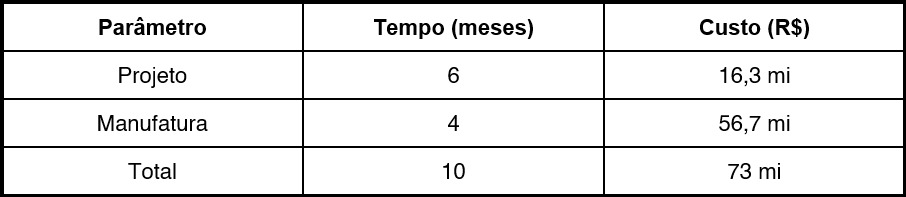
\includegraphics[width=0.8\textwidth]{figuras/tabela1.jpeg}
    \caption{Tempos e custos estimados por etapas}
    \label{fig:tab1}
\end{figure}

\begin{figure}[!ht]
    \centering
    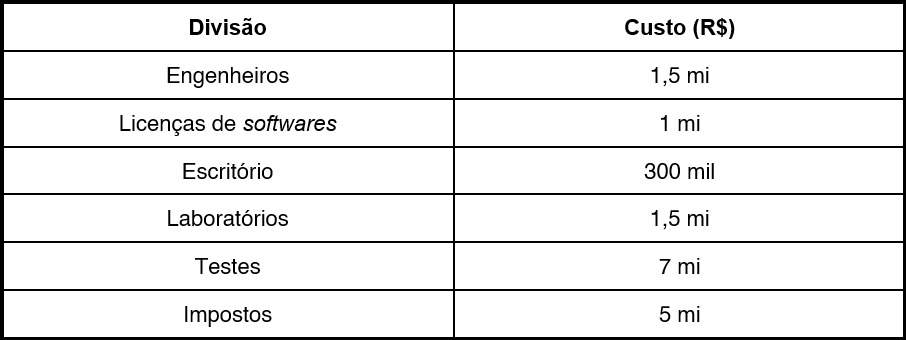
\includegraphics[width=0.8\textwidth]{figuras/tabela2.jpeg}
    \caption{Custos da etapa de projeto}
    \label{fig:tab2}
\end{figure}

\begin{figure}[!ht]
    \centering
    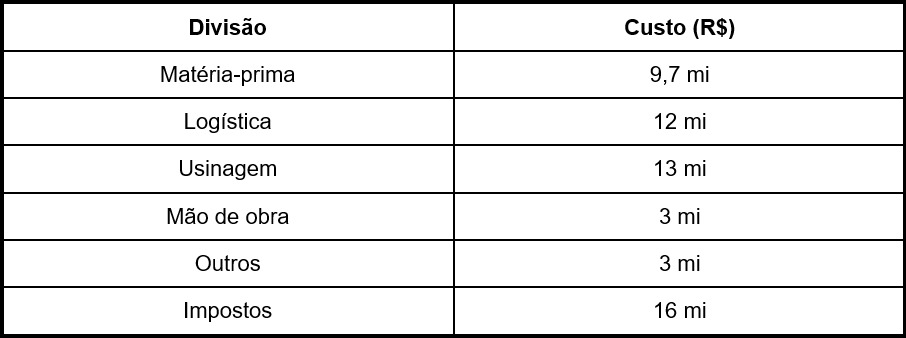
\includegraphics[width=0.8\textwidth]{figuras/tabela3.jpeg}
    \caption{Custos da etapa de manufatura}
    \label{fig:tab3}
\end{figure}

Com as estimativas de custo e tempo realizadas, fez-se um gráfico de custo e lucro por mês para estimar os parâmetros financeiros citados anteriormente.

\begin{figure}[!ht]
    \centering
    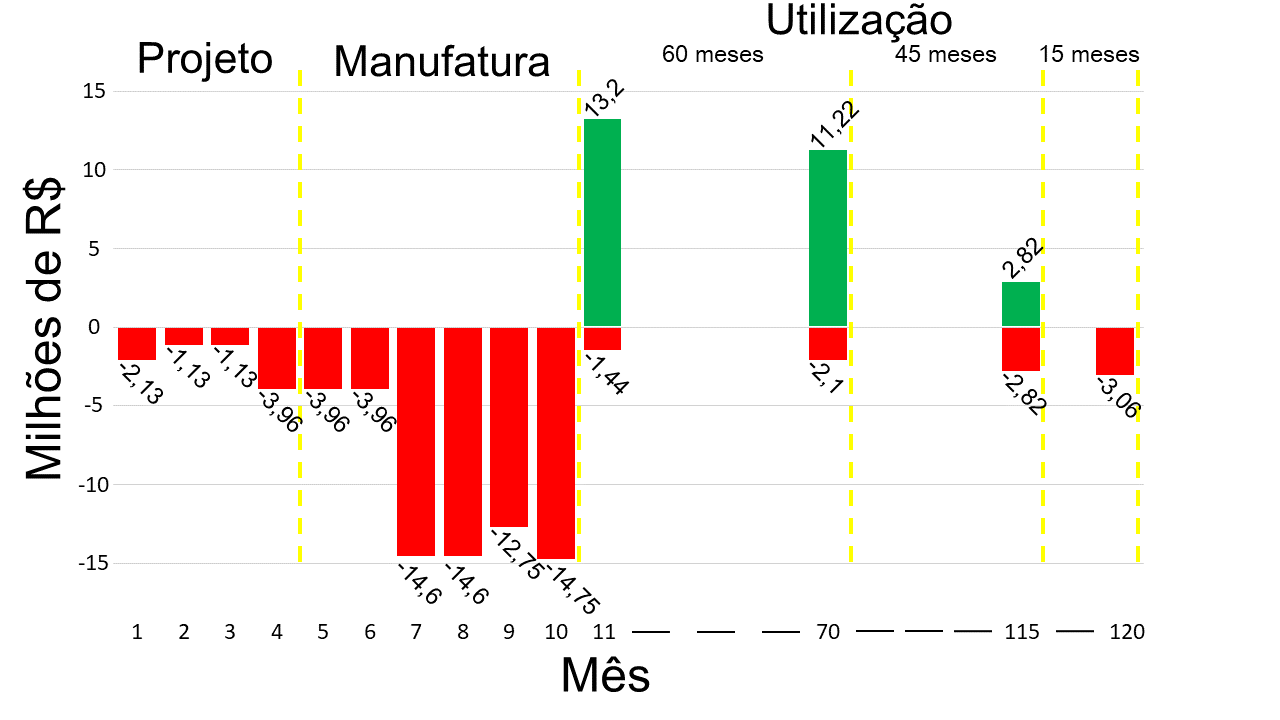
\includegraphics[width=0.8\textwidth]{figuras/img5.png}
    \caption{Custos e lucros ao longo do tempo}
    \label{fig:img5}
\end{figure}

Neste gráfico, observa-se que no primeiro mês do projeto há um custo elevado devido às licenças de softwares, após isso há uma redução no custo por dois meses. Com isso, há um aumento de custo devido aos testes, seguidos pelo início da manufatura e, consequentemente, compra de matéria-prima, usinagem e etc. Por fim, no período de manufatura ainda há grandes custos como logística de transporte da turbina até o local.
Com a instalação da turbina, há um lucro que progressivamente decai por conta da redução de eficiência devido ao desgaste. Após 105 meses, o lucro se torna equivalente aos custos de operação. Dessa forma, após esse tempo de uso, a turbina gerará apenas prejuízo.
Com o gráfico de custos e lucros por tempo, foi possível realizar os cálculos dos parâmetros financeiros. Para isso, foram feitas estimativas, assim, para o custo da turbina e gerador levou-se em consideração a proporção de custo e potência entre a turbina e gerador utilizados na hidrelétrica de Itaipu e os utilizados neste projeto, já a tarifa de transmissão de energia foi estimada considerando as médias de venda de energia em leilões, enquanto o \textit{CAPEX}, \textit{OPEX} e \textit{payback} foram obtidos ao observar o gráfico anterior. Por fim, para a depreciação, VPL e TIR foram utilizadas as seguintes equações:

\[Depreciacao = \dfrac{1}{Vida util}100\%\]

\[ VPL = \sum_{j=1}^{n}\dfrac{FCj}{(1+TMA)^j} - Investimento \; inicial  \], sendo FC o fluxo de caixa, TMA a taxa mínima de atratividade e j o período de cada fluxo de caixa.

\[ TIR = \sum_{t=0}^{n}\dfrac{FCt}{(1+TIR)^t}  \], sendo FC o fluxo de caixa e t o tempo de análise.

\begin{figure}[!h]
    \centering
    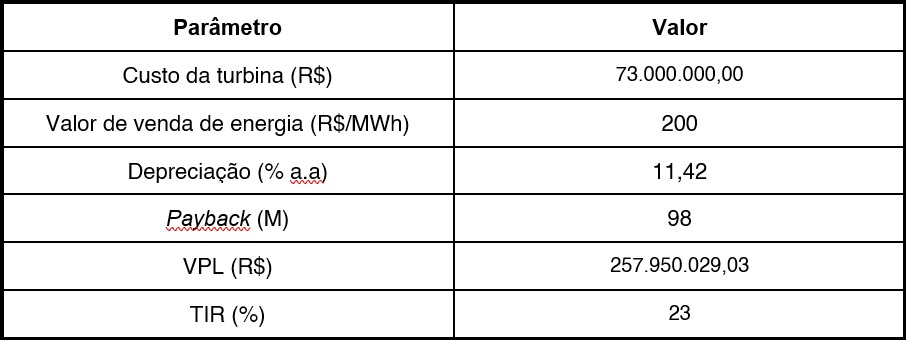
\includegraphics[width=0.8\textwidth]{figuras/tabela4.jpeg}
    \caption{Parâmetros financeiros}
    \label{fig:tab4}
\end{figure}
